\chapter{CONTRATOS REST COM DESIGN-BY-CONTRACT}

 
\section{EXTENSÃO DA NEOIDL PARA DESIGN BY CONTRACT}
\label{extensaoNeoIDL-DbC}

Influência de Eiffel, JML e Spec\#

Eiffel assertions are Boolean expressions, with a few extensions such as the old
notation. Since the whole power of Boolean expressions is available, they may
include function calls. Because the full power of the language is available to
write these functions, the conditions they express can be quite sophisticated.
\cite{meyer1992applying}

 
 
\subsection{Proposta: Serviços com Desing-by-Contract}
\vspace{-6mm}

Os benefícios esperados pela adoção da arquitetura orientada a serviços
somente serão auferidos com a concepção adequada de cada serviço. 
Por essa razão, é necessário planejar o projeto dos serviços criteriosamente
antes de lançar mão do desenvolvimento, com preocupação especial em garantir
um nível aceitável de estabilidade aos consumidores de cada serviço.
Nessa etapa do projeto de desenho da solução, a especificação do contrato do
serviço (Web API) exerce uma função fundamental. 

Na sociedade civil, contratos são meios de se formalizar acordo entre partes a
fim de definir os direitos e deveres de cada parte e buscar atingir o
objetivo esperado dentro de determinadas regras. Cada parte espera que as outras
cumpram com suas obrigações.
Por outro lado, sabe-se que o descumprimeto das obrigações costuma implicar de
penalizações até o desfazimento do contrato. 

Contratos entre serviços Web seguem em uma linha análoga. O desenho das
capacidades (operações) e dos dados das mensagens correspondem aos
termos do contrato no sentido do que o consumidor deve esperar do serviço
provedor. Porém identificou-se, após ampla pesquisa realizada sobre o tema, que
as linguagens disponíves para especificação de contratos atingem apenas esse
nível de garantias. No contexto de webservices em REST, conforme descrito na
seção \ref{secaoREST}, há ainda a ausência de padrão para especificação
contratos, tal como ocorre com o WSDL adotado em SOAP.

A proposta deste trabalho é extender os níveis de garantias, de modo a promover
um patamar adicional com obrigações mutuas entre os serviços (consumidor e
provedor). Isso se dá para adoção do conceito de Design-by-Contract (debatido
na seção \ref{Design-by-Contract}) em que a execução da
capacidade do serviço garantirá a execução, desde que satisfeitas as condições
prévias. O detalhamento do processo é exposto nas seções que se seguem.

\vspace{-6mm}

\subsubsection{Modelo de operação}
\vspace{-6mm}

As garantias para execução dos serviços são estabelecidas em duas etapas: pré- e
pós-condições. Nas pré-condições o provedor do serviço estabelece os requisitos
para que o serviço possa ser executado. A etapa de pós-condições tem o papel de
validar se a mensagem de retorno do serviço possui resultados válidos.

O diagrama da Figura \ref{FigServiceDbC} descreve como ocorre a operação das
pré- e pós-condições. O processo se inicia com a chamada à capacidade do serviço e a
identificação da existência de uma pré-condição. Caso tenham sido estabelecidas 
pré-condições, essas são avaliadas. Caso alguma delas não tenham sido
satisfeitas, o serviço principal não é processado e o provedor do serviço
retornar o código de falha definido no contrato correspondente.


\begin{figure}[!htb]
\centering
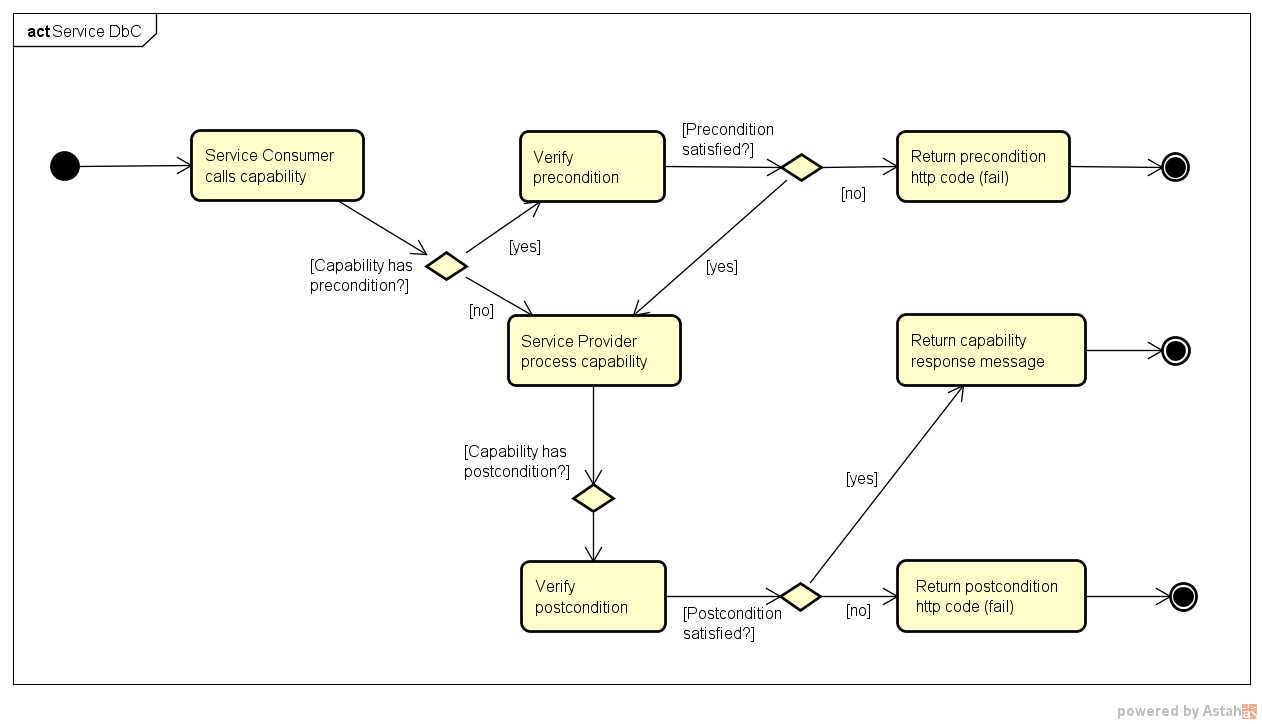
\includegraphics[width=\textwidth,trim = 0mm 5mm 0mm 0mm,clip]{ServiceDbC.png}
\caption{Digrama de atividades com verificação de pré e pós condições}
\label{FigServiceDbC}
\end{figure}

Caso tenham sido definidas pós-condições, essas são acionadas após o
processamento da capacidade, porém antes do retorno ao consumidor do serviço.
Assim, conforme Figura \ref{FigServiceDbC}, visando não entregar ao cliente uma
mensagem ou situação incoerente, as pós-condições são validadas. Caso todas as
pós-condições tenham sido satisfeitas, a mensagem de retorno é encaminhada ao
cliente. Caso contrário, será retornado o código de falha.


\vspace{-6mm}


\subsubsection{Verificação das pré-condições}
\vspace{-6mm}

As pré-condições podem ser do tipo baseado nos parâmetros da requisição ou do
tipo baseado na chamada a outro serviço. Denominamos, para o contexto desta
dissertação, de básica a pré-condição baseada apenas nos parâmetros da
requisição (atributos da chamada ao serviço). Nessa validação é direta,
comparando os valores passados com os valores admitidos. 

No caso das pré-condições baseadas em serviços, é realizada chamada a outro
serviço para verificar se uma determinada condição é satisfeita. Este modo de
funcionamento, que se assemelha a uma composição de serviço, é mais versátil, pois permite
validações de condições complexas sem que a lógica associada seja conhecida pelo
cliente. Assim, os contratos que estabelecem esse tipo de
pré-condição se mantem simples.

A Figura \ref{FigServicePrecondition} detalha as etapas de verificação de cada
pré-condição. Nota-se que a saída para as situações de desatendimento às
pré-condições, independentemente do tipo, é o mesmo. O objetivo desta abordagem
é simplificar o tratametno de exceção no consumidor.

\begin{figure}[!htb]
\centering
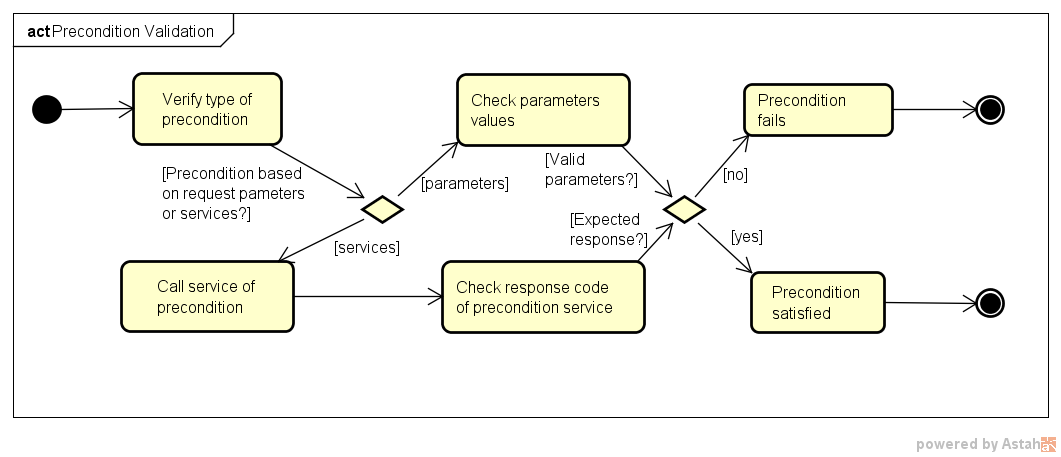
\includegraphics[width=\textwidth,trim = 0mm 5mm 0mm 0mm,clip]{PreconditionValidation.png}
\caption{Diagrama de atividades do processamento da pré-condição}
\label{FigServicePrecondition}
\end{figure}


\subsubsection{Verificação das pós-condições}
\vspace{-6mm}

\begin{figure}[!htb]
\centering
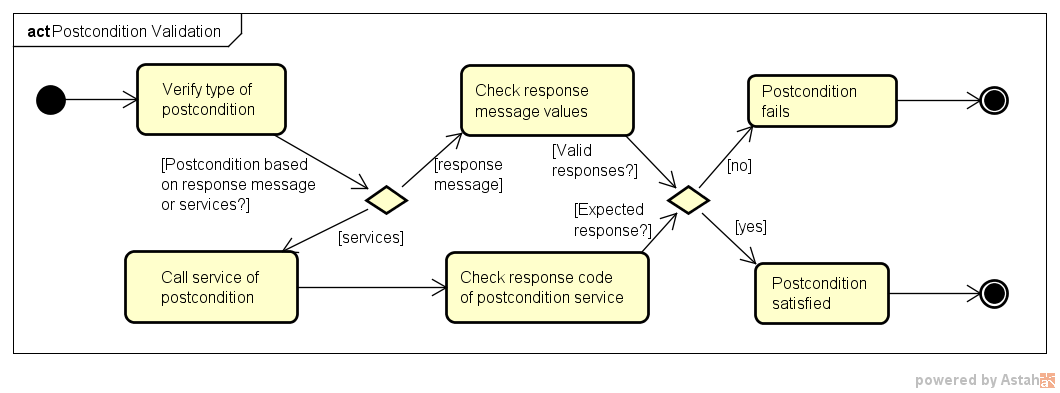
\includegraphics[width=\textwidth,trim = 0mm 5mm 0mm
0mm,clip]{PostconditionValidation.png} 
\vspace{-6mm}
\caption{Diagrama de atividades do processamento da pós-condição}
\label{FigServicePostcondition}
\end{figure}

A verificação das pós-condições acontece de modo muito similar a das
pré-condições. Há também os dois tipos, baseado em valores e em chamadas a
outros serviços. O diferencial está em que a validação dos valores passa a
ocorrer a partir dos valores contidos na mensagem de retorno. A Figura
\ref{FigServicePostcondition} descreve as etapas necessárias para validação de
cada pré-condição.

	
	
	
	

\subsection{Extensão da linguagem}

\subsubsection{Precondição básica}

\begin{figure}[htb]
\begin{small}
\lstinputlisting[language=NeoIDL,firstnumber=1]{DBCsimple.neo}
\end{small}
\caption{Exemplo da notação DBC básica na \neoidl{}}
\label{lst:DBCService}
\end{figure} 

\subsubsection{Pós-condição básica}

\ldots



\subsubsection{Precondição com chamada a serviço}

\begin{figure}[htb]
\begin{small}
\lstinputlisting[language=NeoIDL,firstnumber=1]{DBCservice.neo}
\end{small}
\caption{Exemplo da notação DBC na \neoidl{} com chamada a serviço}
\label{lst:DBCService}
\end{figure} 


\subsubsection{Pós-condição com chamada a serviço}

\ldots

\subsection{Estudo de caso: plugin twisted}
\label{pluginTwisted}

\ldots

\subsubsection{Arquitetura}

% Diagrama da estrutura do código gerado


\subsubsection{Geração de código}

\section{ESTUDO EMPÍRICO DA ANÁLISE SUBJETIVA}
\vspace{-6mm}

\label{analiseSubjetiva}
\vspace{-6mm}

%%%%
A language's expressiveness is the major criterion for choosing a language to
state a given set of facts: a language that cannot express the facts should not
be used. However, additional criteria are needed to choose among languages that
are sufficiently expressive  for a set of facts. Two of these criteria are how
ease it is to state the facts in the language and how easy is to perceive the
facts once they are stated.

expressividade de uma linguagem é o principal critério para a escolha de uma
linguagem para indicar um determinado conjunto de fatos: uma linguagem que não
podem expressar os fatos não devem ser usados. No entanto, os critérios
adicionais são necessários para escolher entre os idiomas que são
suficientemente expressivo para um conjunto de fatos. Dois desses critérios são
quão fácil é expor os fatos na linguagem e como é fácil de perceber os fatos,
uma vez que são demonstrados.

\cite{mackinlay1985expressiveness}

%%%%


%%%
Instead of aiming to be the best for solving any kind of
computing problem, DSLs aim to be particularly good for
solving a specific class of problems, and in doing so they
are often much more accessible to the general public than tra-
ditional programming languages.
\cite{taha2008domain}
%%%% 

%%%%
They offer substantial gains in expressiveness and ease of use compared
with GPLs in their domain of application’. [2] describes the typical costs of a
DSL, noting that a small extra initial investment in a DSL implementation typ-
ically leads to long term savings, in comparison to alternative routes.
\cite{tratt2008evolving}
%%%%

%%%%
A domain specific language (DSL) is a program-
ming language tailored for a particular application do-
main. Characteristic of an effective DSL is the ability
to develop complete application programs for a do-
main quickly and effectively. A DSL is not (neces-
sarily) “general purpose.” Rather, it should capture
precisely the semantics of an application domain, no
more and no less.

There are lots of advantages to using DSLs, start-
ing with the fact that programs are generally easier to
write, reason about, and modify compared to equivalent 
programs written in general purpose languages.
Indeed, these are the same advantages gained from using any high-level
programming language.
\cite{hudak1998modular}
%%%%




\subsection{Método}
\vspace{-6mm}

\subsection{GQM}
\vspace{-6mm}

\subsection{Questionário}
\vspace{-6mm}

\subsection{Análise dos Resultados}
\vspace{-6mm}


* Questionário montado para avaliar a utilidade de DbC com NeoIDL

* Inicialmente motivado pelo estudo do Alessandro Garcia

* GQM e Avaliação TAM

* Montagem do questionário

1. Perfil técnico-profissional do respondente
1.1 Para qual órgão ou empresa você presta serviços atualmente?
1.2 A quanto tempo você trabalha com desenvolvimento Web
1.3 A quanto tempo você desenvolve com uso de APIs Web (Web Service)
1.4 Qual o seu nível de experiência com especificação de API REST
1.5 Qual o seu nível de experiência com especificação de contratos com Swagger

3 Questões sobre especificação e implementação de APIs Web
3.1 A especificação do contrato formalmente, seja em Swagger ou NeoIDL, em
relação a descrição textual, aumentará meu nível de acerto na implementação (efetividade).
3.2 Identificar e compreender as operações e atributos na especificação Swagger
é simples para mim.
3.3 Identificar e compreender as operações e atributos na especificação NeoIDL é
simples para mim.

4. DbC
4.1 Conhecer previamente e explicitamente as pré-condições será útil para mim.
(Useful)
4.2 Aprender a identificar as pré-condições na NeoIDL parece ser simples pra mim
(Easy to learn)
4.3 Parece ser fácil para mim declarar uma pré-condição na NeoIDL
(Clear and understandable)
4.4 Me lembrar da sintaxe da pré-condição na NeoIDL é fácil  (Remember)

5. Geração de código
5.1 É claro e compreensível para mim o efeito da pré-condição sobre o código
gerado  (Controllable)
5.2 A geração do código de pré e pós-condições aumentará minha produtividade na
implementação do serviço (Job performance)
5.3 Assumindo ter a disposição a NeoIDL no meu trabalho, para especificação de
contratos e geração de código, eu presumo que a utilizarei regularmente no futuro.
5.4 Nesse mesmo contexto, eu vou preferir utilizar contratos escritos em NeoIDL
do que descritos de outra forma



* Distribuição do questionário

* Avaliação dos resultados

* Ameaças
- não foi fornecido nenhum material sobre a NeoIDL, apresentando somente o uma
descrição de serviço
- O questionário foi aplicado uma única vez, sem melhorias a partir do primeiro
conjunto de respostas


* Questionários futuros

A principal questão de pesquisa a ser avaliada com o uso do questionário é a utilidade em se agregar ao design das especificações de serviços REST as garantias de pré e
pós-condições. Em segundo momento, pressupondo a utilidade, avaliar se a NeoIDL
cumpre satisfatoriamente com este propósito, agregando à sintaxe da linguagem
a possibilidade de se expressar pré e pós-condições.

* Separar os respondentes em faixas de experiência. Verificar se as respostas
dos menos experientes precisam ser descartadas pela pouca capacidade crítica.
Separar a análise entre os respondentes que conhecem e os que não conhecem
Swagger.

* Perspectivas de comparação
a) Experiência com desenvolvimento com uso de REST
b) Experiência com Swagger
c) Utilidade da especificação formal de contratos
d) Percepção da NeoIDL sem DbC





